In diesem Abschnitt sollen verschiedene Ma{\ss}nahmen gegen Cyber Sickness vorgestellt werden. Dar\"uberhinaus soll erkl\"art werden, warum diese wirkungsvoll sind und was m\"ogliche Nachteile bei der Nutzung entsprechder Ma{\ss}nahmen sein k\"onnten.

Die Ma{\ss}nahmen lassen sich in auf Grund der Sensory Conflict Theory in drei Kategorien einteilen: 
Reduktion der Inkongruenz der visuellen Reize entgegen der Erfahrung, indem diese optimiert werden (\autoref{Visuals}), Generation von kongruenten, vestibul\"aren Stimuli entsprechend der Erwartung durch die visuellen Reize (\autoref{Vestibular}) und Adaptation durch den Organismus selbst, unter Beachtung bestimmter Faktoren (\autoref{Adaptation}). Eine generell zu erkennende Tendenz besteht darin, dass diese Methoden versuchen, eine gewohnte \textbf{Nat\"urlichkeit} in der virtuellen Umgebung zu erzeugen.

\subsection{Anpassung der visuellen Reize}\label{Visuals}
Eine Vection passiert dann, wenn ein \textbf{statischer Referenzpunkt} fehlt, an dem man sich optisch fixieren und somit seine Lage relativ dazu sicher feststellen kann. Dies passiert beispielsweise, wenn man aus einem Zug auf einen anderen schaut, ohne den Himmel sehen zu k\"onnen. Wenn der andere Zug sich in Bewegung setzt, erlebt man kurzzeitig Vection, da hier der Himmel als statische Referenz fehlte.

Daher kann ein unabh\"angiger Hintergrund, vorrangig bei CAVE Displays, nach Duh und Parker \cite{Duh:2001:Static} helfen. Nat\"urlich ist die Methoden beispielsweise bei Head-Mounted Displays nicht nutzbar, da diese die visuelle Wahrnehmung der tats\"achlichen Umgebung vollst\"andig ersetzen. Eine Methode dennoch einen bekannten Fixpunkt in die virtuelle Umgebung zu integrieren ist die virtuelle Nase wie in \autoref{abb:vnose}, die laut Wienrich et al.\cite{Wienrich:2018:Nose} die Intensit\"at von Cyber Sickness bei Nutzung von Head-Mounted-Displays reduzieren kann.


\begin{figure}[tbh]
	\centering 
	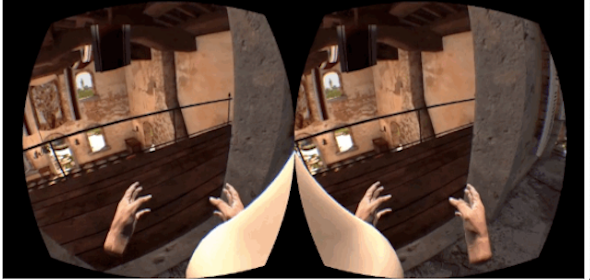
\includegraphics[width=\columnwidth]{virtual_nose.png}
	\caption{Virtuelle Nase zur Reduktion von Cyber Sickness bei Head-Mounted Displays. Bild von WIRED\cite{WIRED:2020:Nose}, letzter Zugriff: 03.05.2020}
	\label{abb:vnose}
\end{figure}


Desweiteren ist es f\"ur die Reduktion von Cyber Sickness ratsam, wenn die graphische Darstellung und Design der virtuellen Umgebung sich dadurch auszeichnen, dass sie nat\"urlich wirken und ruhige, weite Szenen ohne schnellwechselnde Bewegungen nachbildet. Die Parameter der Graphik sollten wie folgt umgesetzt werden:

Die Aufl\"osung und Wiederholungsrate\footnote{50-60 Hz, nach Davis et al.\cite{Davis:2014:Factors}} sollten angemessen hoch sein\cite{kirollos:2019:refresh}, das \textit{Field of View} sollte sich nach Fernandes und Feiner\cite{Fenandes:2016:FOV} dynamisch anpassen und tendenziell eher klein sein und hoch \"uber dem Boden ansetzen, sofern der Kontext, f\"ur den die virtuelle Umgebung genutzt wird, das zul\"asst. Geringe Latenz f\"uhrte nach Meehan et al.\cite{Meehan:2003:latency} zu mehr wahrgenommener Presence und laut Davis et al.\cite{Davis:2014:Factors} auch zu Cyber Sickness, ebenso wie durch Flickern in der Darstellung der virtuellen Umgebung.
Bei all diesen Punkten stellt sich immer die Frage des Aufwandes und der Umsetzbarkeit durch die verf\"ugbare Hardware.

Es scheint, als verursachen realistischere Graphik bzw. Animationen st\"arkere Cyber Sickness\cite{Pouke:2018:Realism}.
In Anbetracht der beiden Punkte, statische Referenz und Nat\"urlichkeit, empfehlen sich weite Landschaften in virtuellen Umgebungen und im Sinne der Sensory Conflict Theory, Fortbewegung in Virtual Reality m\"oglichst zu reduzieren\footnote{In Computerspielen zum Beispiel Teleportation nutzen}, wobei sich hier erneut das Problem aufwirft, dass diese Methoden nicht in jedem Kontext einsetzbar sind.

Obwohl mit den genannten Anpassung der visuellen Komponente die Vection schon wesentlich angenehmer und weniger gest\"ort durch Cyber Sickness sein kann, sodass auch eine Immersion in die virtuelle Umgebung stattfindet, ist es immer m\"oglich zus\"atzlich kongruente, vestibul\"are Stimuli zu erzeugen, sodass die Vection keine Illusion mehr ist, sondern nahe an das tats\"achliche Bewegungserlebnis herankommt.


\subsection{Erzeugen kongruenter Stimuli}\label{Vestibular}

Zu den visuellen Reizen der virtuellen Umgebung k\"onnen die verschiedenen Sinneskan\"ale kongruente Stimuli erg\"anzen, auch durch auditive oder haptische, um die Orientierung im virtuellen Raum zu erh\"ohen. Vorrangig l\"asst sich Cyber Sickness aber reduzieren, indem man eine entsprechende M\"oglichkeit der Bewegung einr\"aumt, w\"ahrend man in der virtuellen Umgebung ist. Dies ist vor allem durch sogenannte VRN-Chairs und Treadmills m\"oglich.

VRN-Chairs sind Rollst\"uhle, die mit magnetischen Sensoren ausgestattet werden, sodass die Bewegung der R\"ader des Rollstuhls passend in die Virtual Reality \"ubertragen werden kann. Durch gleichgerichtete Drehung der R\"ader kann eine Vor- oder R\"uckw\"artsbewegung, durch entgesetzte Drehnung eine Rotation in die jeweilige Richtung erzeugt werden. Durch das unterschiedlich starkes Drehen k\"onnen Kurven gefahren werden. Laut Byagowi\cite{Byagowi:2014:VRNchair} reduzieren VRN-Chairs Cyber Sickness und haben den Vorteil, dass sie barrierefrei sind, sodass sie auch in speziellen medizinischen Szenarien genutzt werden k\"onnen. Generell treten im Sitzen in Virtual Reality weniger Symptome von Cyber Sickness auf. Der Nachteil von VRN-Chairs liegt in Anwendungen, welche die die dritte Dimension in der virtuellen Umgebung stark beanspruchen.

Eine weitere M\"oglichkeit der Lokomotion in der virtuellen Realit\"at sind Treadmills. Diese sind in der Regel omnidirektional, sodass Bewegung in alle Richtungen m\"oglich ist. Nach Aldaba und Moussavi\cite{Aldaba:2019:VRNTread} sind VRN-Chairs gegen\"uber Treadmills effektiver, da sie den Reizen der nat\"urlichen Bewegung eher entsprechen unddadurch die Symptome der Cyber Sickness weniger intensiv sind, wie in \autoref{abb:comp_vrn_tread} zu sehen ist. Desweiteren beantspruchen Treadmills oft viel Raum. Au{\ss}erdem sind sie gegen\"uber VRN-Chairs nicht barrierfrei und wesentlich kostenintensiver.
\begin{figure}[h]
	\centering 
	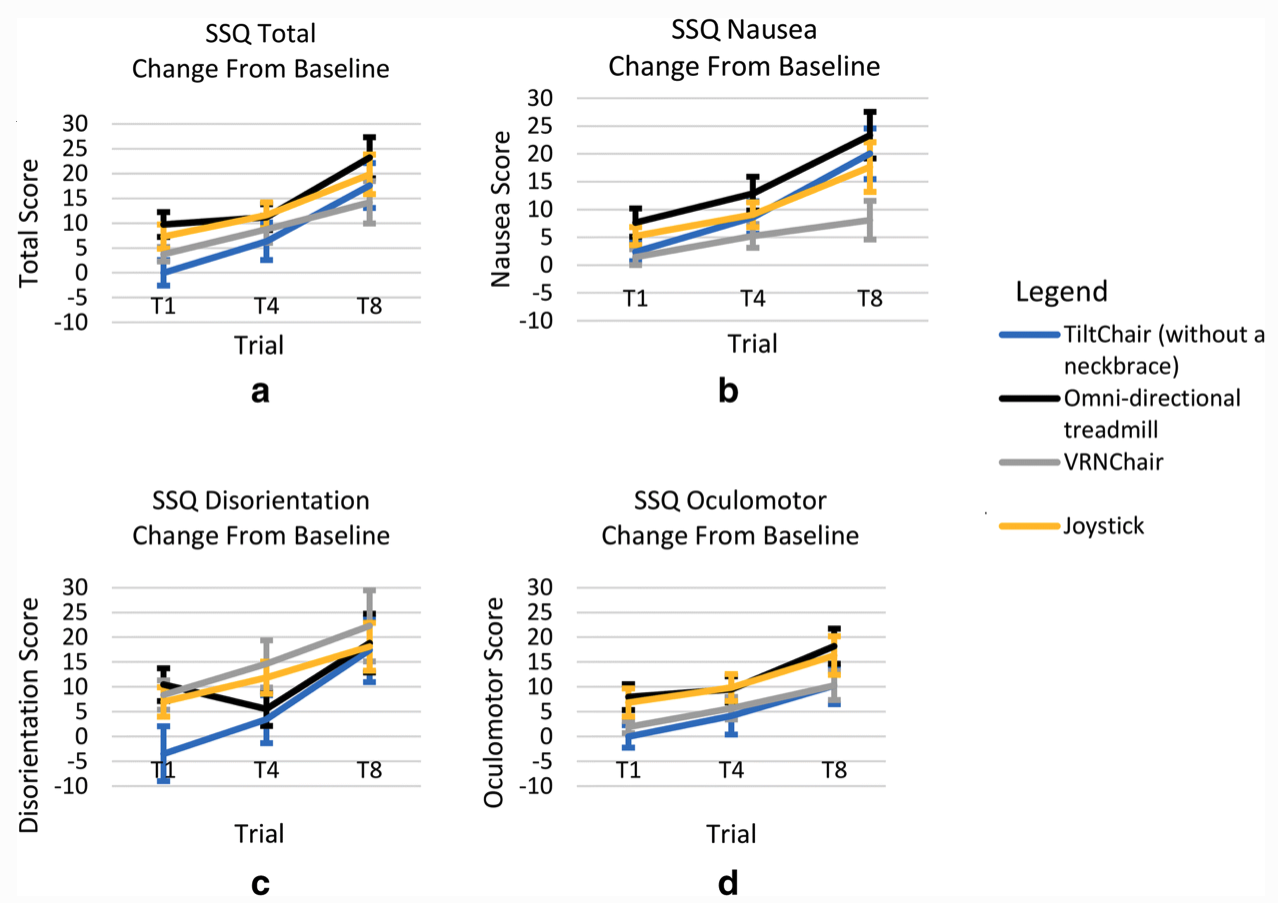
\includegraphics[width=\columnwidth]{comparision_vrn_tread.png}
	\caption{Vergleich verschiederer Methoden bez\"uglich Cyber Sickness von Aldaba und Moussavi\cite{Aldaba:2019:VRNTread}. Niederige SSQ-Scores bedeuten weniger Cyber Sickness.}
	\label{abb:comp_vrn_tread}
\end{figure}

Ohne eine tats\"achlich stattfindende Bewegung, die dann durch die Tr\"agheit der Fl\"ussigkeit in den Bogeng\"angen des Innenohrs einen Reiz erzeugt, funktioniert die \textit{galvanische Vestibul\"arstimulation}, bei der das Gleichgewichtsorgan nicht-invasiv direkt stimuliert wird. Nach Weech et al.\cite{Weech:2020:GVS} kann sie kurzzeitig Cyber Sickness reduzieren, w\"ahrend und kurz nach der Reizung.
Galvanischen Vestibul\"arstimulation scheint effektiv zu sein, weil der Organismus in der virtuellen Umgebung die Gewichtung der Sinneskan\"ale neu bestimmt. Vestibul\"are Reize werden als unzuverl\"assig empfunden und es finden ein \textit{Down-Weighing} statt, wogegen sich mehr auf die visuellen Stimuli verlassen wird und diese st\"arker gewichtet werden.
Der Nachteil dieses Verfahrens ist, dass es noch relativ unerforscht ist und Auswirkungen auf h\"ohere kognitive Schichten unbekannt sind.


Wenn ein Organismus sich nach so kurzer Zeit schon anzupassen beginnt, stellt sich die Frage, wie die Adaptation nach l\"angerer Zeit mit regelm\"a{\ss}iger Nutzung aussieht und welche weiteren Faktoren das Auftreten von Cyber Sickness noch beeinflussen k\"onnen.

\subsection{Adaptation und interindividuelle Faktoren}\label{Adaptation}

Damit eine Anpassung an virtuelle Realit\"aten gelingt, ist es wichtig zu wissen, welche Faktoren \"uber die Inkongruenz der visuellen und vestibul\"aren Stimuli hinaus daf\"ur eine mediierende Rolle haben, sodass man durch die Art und Weise wie und bei wem Virtual Reality genutzt wird, die Adaptation erleichtern kann.

Je l\"anger die sukzessiv verbrachte Zeit in einer virtuellen Realit\"at w\"ahrend einer Session, desto intensiver werden die Symptome der Cyber Sickness\cite{Aldaba:2017:VRNTreadGraphic}, wie auch in \autoref{abb:comp_vrn_tread} deutlich wird. Werden mehr Versuche am St\"uck durchgef\"uhrt werden, so erh\"ohen sich die Scores des SSQ. LaViola\cite{LaViola:2000:CSinVR} konnte zeigen, dass eine Gew\"ohnung an die Virtual Reality stattfindet und sich \"uber mehrere Sessions hinweg so die Cyber Sickness reduziert.
Durch Langzeitpotenzierung ver\"andern Neuronen, was als Lernen bezeichnet wird. 

Wie bereits von der bei galvanischen Vestibul\"arstimulation bekannt ist, kann innerhalb einer Session eine ver\"anderte Verarbeitung der Reize stattfinden, was offenbar auch bleibende Effekte hat. Also lernt man, mit der neuen Situation in der virtuellen Realit\"at umzugehen.
Es empfiehlt sich daher, mit kurzen Sessions zu beginnen und die L\"ange sukzessiv zu erh\"ohen, um dem Organismus Zeit zu geben, sich anzupassen und wenig Belastung durch die Symptome der Cyber Sickness zu verursachen.
Hier muss man sich die Frage stellen, ob der Kontext, in welchem die Virtual Reality genutzt werden soll, genug Zeit f\"ur eine Gew\"ohnungsphase einr\"aumt.

Ein weiterer Faktor ist die Kontrolle, die man in der virtuellen Umgebung hat\cite{Kolasinski:1995:control}. Dies liegt daran, dass sich bestimmte Sinneswahrnehmungen erahnen lassen, wenn man in der virtuellen Umgebung selbst bestimmen kann, was als n\"achstes passiert. Im Sinne der Theorie, dass Motion Sickness einen evolution\"aren Vergiftungsschutz darstellt, ist dieser Faktor sinnvoll. Nervengifte erzeugen nicht nur eine Inkongruenz zwischen den verschiedenen Sinnen, sondern l\"ahmen auch Muskeln, sodass man keine Kontrolle mehr hat. Daher reagiert der K\"orper mit intensiv, was die Symptome der Cyber Sickness zur Folge hat.

Davis et al.\cite{Davis:2014:Factors} nennen eine Reihe interindividueller Faktoren: Alter, Krankheit, Haltung und Geschlecht. Kinder besitzen danach die h\"ochste Anf\"alligkeit f\"ur Cybersickness, was sich mit zunehmendem Alter reduziert. Die Fl\"ussigkeit der Bogeng\"ange des Innenohrs wird ebenfalls mit zunehmendem Alter viskoser, sodass die vestibul\"areren Stimuli weniger intensiv sind, was wiederum zu weniger Inkongruenz mit den visuellen Reizen f\"uhrt.

Generelle gesundheitliche Probleme, Erkrankungen sowie Alkohol- und Drogenkonsum\cite{Kruk:1992:Drugs} erh\"ohen ebenfalls die Anf\"alligkeit f\"ur Cyber Sickness. Zur Haltung gilt zu sagen, dass Leute mit einer stabileren Haltung weniger unter Cyber Sickness leider als solche mit einer instabilen. Au{\ss}erdem f\"uhrt Virtual Reality im Sitzen ausgef\"uhrt zu weniger Symptomen als stehend.

Geschlecht gilt als weiterer Faktor. Tendenziell leiden Frauen eher an Cyber Sickness als M\"anner\cite{Aldaba:2019:VRNTread}. Frauen scheinen ein weiteres Field of View zu haben, was Cyber Sickness erh\"oht, wie in \autoref{Vestibular} erkl\"art wurde. Dar\"uberhinaus k\"onnen weibliche Hormone die Anf\"alligkeit erh\"ohen\cite{Kolasinski:1995:control}.


Ein letzter Faktor, der die Adaptation erschweren k\"onnte, ist die Passform des technischen Equipments f\"ur den Anwender, mit dem virtuelle Realit\"aten dargestellt werden - insbesondere bei HMD\footnote{Akronym von Head-Mounted Display}. Der Pupillenabstand bei Menschen folgt einer Normalverteilung, jedoch ist der Abstand bei M\"annern durchschnittlich h\"oher als bei Frauen und die aktuelle Standardgr\"o{\ss}e entspricht im Mittel eher der interpupillaren Distanz bei M\"annern\cite{UploadVR:2020:HMDfit}, sodass die Nutzung im Verh\"altnis f\"ur M\"annern angenehmer ist, ersichtlich in \autoref{abb:hmdfit}. 
\begin{figure}[h]
	\centering 	
	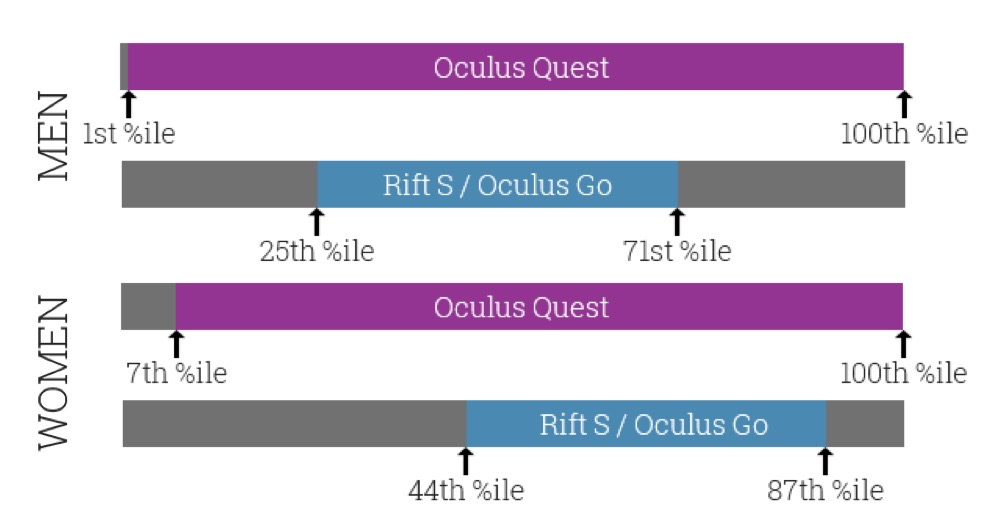
\includegraphics[width=\columnwidth]{fitting.jpeg}
	\caption{Perzentile erwachsener M\"annern und Frauen f\"ur die das jeweilige HMD anhand des Pupillenabstandes am besten geeignet ist. Rift S besitzt einen festen Abstand, im Gegensatz zu Oculus Quest. Bild von UploadVR\cite{UploadVR:2020:HMDfit}, letzter Zugriff: 04.05.2020}
	\label{abb:hmdfit}
\end{figure}


Dieser Faktor k\"onnte auch eine Erkl\"arung f\"ur einige der interindivduelle Faktoren sein, insbesondere Alter und Geschlecht. Da die Erfahrung durch eine schlechte Passform des Head-Mounted Displays wesentlich unnat\"urlicher - allein von einem visuellen Aspekt - f\"ur den Anwender ist, treten Symptome von Cyber Sickness auf.





